%%%%%%%%%%%%%%%%%%%%%%%%%%%%%%%%%%%%%%%%%
%
% (c) 2019 by Jennifer Laaser
%
% This work is licensed under the Creative Commons Attribution-NonCommercial-ShareAlike 4.0 International License. To view a copy of this license, visit http://creativecommons.org/licenses/by-nc-sa/4.0/ or send a letter to Creative Commons, PO Box 1866, Mountain View, CA 94042, USA.
%
% The current source for these materials is accessible on Github: https://github.com/jlaaser/pogil-polymers
%
%%%%%%%%%%%%%%%%%%%%%%%%%%%%%%%%%%%%%%%%%

\renewcommand{\figpath}{content/polymchem/networks/network-stepgrowth/figs}
\renewcommand{\labelbase}{network-stepgrowth}

\begin{activity}[extension]{Synthesis of Polymer Networks by Step-Growth Reactions}

\begin{instructornotes}
	This activity introduces students to concepts related to the synthesis of polymer networks by step-growth polymerization.
	
	After completing this activity, students will be able to:
	\begin{enumerate}
		\item Explain how multifunctional monomers can be used to synthesize polymer networks by step-growth polymerization
		\item Calculate the extent of reaction necessary to form a polymer network in a stoichiometrically-balanced reaction
	\end{enumerate}
	
	Note that this activity can be completed any time after the activity on molecular weight and stoichiometry in step-growth polymerizations; it \emph{does not} rely on any concepts from the molecular weight and dispersity activity.
	
	\subsection*{Activity summary:}
	\begin{itemize}
		\item \textbf{Activity type:} Learning Cycle
		\item \textbf{Content goals:} See above
		\item \textbf{Process goals:} %https://pogil.org/uploads/attachments/cj54b5yts006cklx4hh758htf-process-skills-official-pogil-list-2015-original.pdf
			\begin{enumerate}
				\item Linking concepts to derive a key result
				\item Communication (written and oral) of reasoning
			\end{enumerate}
		\item \textbf{Duration:} 25 minutes, including time for class discussion
		\item \textbf{Instructor preparation required:} none beyond knowledge of relevant content
		\item \textbf{Related textbook chapters:}
			\begin{itemize}
				\item \emph{Polymer Chemistry} (Hiemenz \& Lodge), 2nd ed.: section 10.2
				\item \emph{Introduction to Polymers} (Young \& Lovell), 3rd ed.: section 3.3
			\end{itemize}
		%\item \textbf{Facilitation notes:}
		%	\begin{itemize}
		%		\item \dots
		%	\end{itemize}
	\end{itemize}
	
\end{instructornotes}

\begin{model}[Step-Growth Network Synthesis]

	One way to synthesize a polymer network is via step-growth polymerization of multi-functional monomers.
	
	For example, a step-growth polymerization of a difunctional ``AA'' monomer with a trifunctional ``B$_3$'' monomer might yield a network as follows:
	
	\centerline{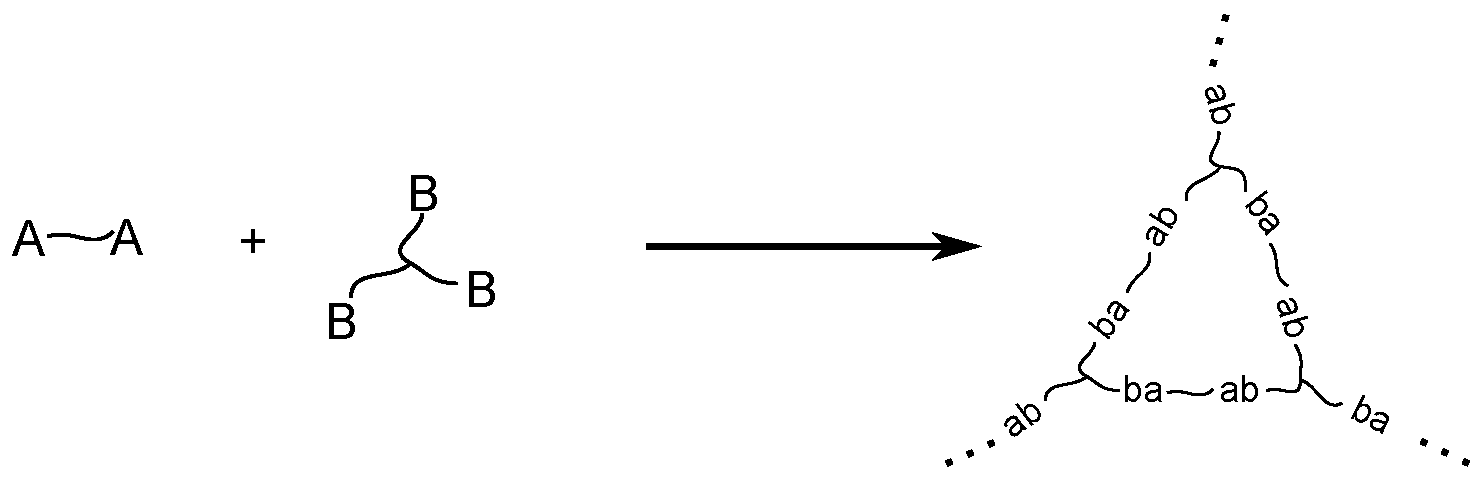
\includegraphics[width=0.8\textwidth]{\figpath/Model2_A2B3network.pdf}}

\end{model}

\begin{ctqs}

	\question Suppose that you started this reaction with three AA-type monomers and two $B_3$ monomers, as shown below:
	
	\vspace{9pt}
		\centerline{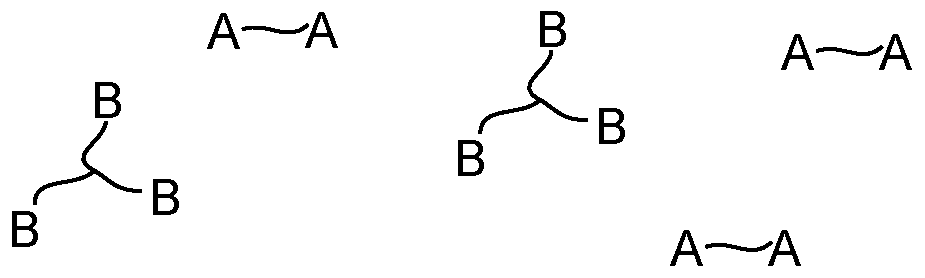
\includegraphics[width=0.5\textwidth]{\figpath/Model2_A2B3_initial.pdf}}
	
		\begin{enumerate}
			\item How many \emph{molecules} are present in the initial reaction mixture?
			
				\begin{solution}[0.5in]{}
					5
				\end{solution}
			
			\item How many \emph{reactive functional groups} are present in the initial reaction mixture?  For the purposes of this question, count both the A and B reactive groups.
			
				\begin{solution}[0.5in]{}
					12 (6 from AA-type monomers, 6 from B\textsubscript{3}-type monomers)
				\end{solution}
				
			\item What is the average number of functional groups \emph{per monomer} in this reaction mixture?
			
				\begin{solution}[0.5in]{}
					12/5 = 2.4
				\end{solution}
			
		\end{enumerate}
	
	\clearpage
	\question Now, suppose we move two ``steps'' forward in the reaction (i.e. we form two ``ab'' bonds).
	
		\begin{enumerate}
		
			\item Draw one possible reaction mixture that could occur after two bond-forming reactions have taken place:
			
				\begin{solution}[1.5in]{}
				
					(student answers may vary)
					
				\end{solution}
			\item How many \emph{molecules} are present in the mixture you drew in part (a)?
			
				\begin{solution}[0.5in]{}
					3
				\end{solution}
				
			\item Recall that the extent of reaction, $p$, is the fraction of ``A'' groups that have reacted at any given time.  Calculate the extent of reaction for the state of the reaction that you drew in part (a).
			
				\begin{solution}[1.25in]{}
					$p = \frac{\text{\# of A groups reacted}}{\text{initial \# of A groups}} = \frac{2}{6} = 0.33$
				\end{solution}
				
			\item Calculate the number-average degree of polymerization by dividing the initial number of molecules by the number of molecules present at this point in the reaction.  Does your answer agree with the value you obtain using $N_n = \frac{1}{1-p}$?  If not, briefly suggest one possible reason for the discrepancy.
			
				\begin{solution}[2in]{}
					$N_n = \frac{\text{initial \# of molecules}}{\text{final \# of molecules}} = \frac{5}{3} = 1.67$
					
					vs.
					
					$N_n = \frac{1}{1-p} = \frac{1}{1-0.33} = \frac{1}{0.67} = 1.5$
					
					These values do not agree - the number-average degree of polymerization is higher for the case of multifunctional monomers.  Student reasoning may vary; reasonable answers include noting that not all of the functional groups on these monomers need to react to continue the polymer chain, or that the multifunctional reaction mixture had fewer molecules to start with than an AA+BB polymerzation would, so the same number of reaction steps incorporates a higher fraction of the molecules into the chains.
				\end{solution}
		\end{enumerate}
\end{ctqs}

\clearpage
\begin{infobox}
	It is possible to show (see Exercise \ref{\labelbase:exc:Nn}) that for a reaction mixture with an average of $\langle f\rangle$ functional groups per monomer, the number-average degree of polymerization at extent of reaction $p$ is
	\begin{equation*}
		N_n = \frac{2}{2-p\langle f \rangle} \label{\labelbase:eqn:carothers}
	\end{equation*}
	This relationship is referred to as the \emph{Carothers equation}.
\end{infobox}

\begin{ctqs}
	\question As the network begins to form, all of the monomers effectively link into a single large molecule.  What must happen to $N_n$ in this case?  Briefly explain your group's reasoning in 1-2 complete sentences.
	
		\begin{solution}[1.5in]{}
			As the monomers all link into a single molecule, $N_n$ must become very large.  In the limit of having a large number of initial monomers, $N_n$ effectively goes to infinity.
			
			\emph{Note: strictly speaking, it is actually $N_w$ that must approach infinity, but this distinction is a subtle point and not necessary for this activity.}
		\end{solution}
	
	\question What must be true about the value of $2-p\langle f \rangle$ in order for $N_n$ to reach the limit you identified in the previous question?
	
		\begin{solution}[1.5in]{}
			$2-p\langle f\rangle = 0$ (value of the fraction blows up if the denominator is zero)
		\end{solution}
	
	\question Rearrange your answer to the previous question to find the minimum extent of reaction at which a network will form.
	
		\begin{solution}[1.25in]{}
			$p = \frac{2}{\langle f \rangle}$
		\end{solution}
\end{ctqs}


\begin{exercises}

%	\exercise Exercise about stoichiometric imbalance in network synthesis?
	
	%\exercise In Model \ref{\labelbase:mdl:linking}, you considered formation of networks by linking together pre-formed polymer chains.  However, the same analysis can be used to understand networks formed by chain-growth polymerization of mixtures containing difunctional monomers.
	
	%	\begin{enumerate}
	%		\item 
	%	\end{enuemrate}	
	
	\exercise Consider the AA+BB-type step-growth polymerizations that you learned about earlier this term.
	
		\begin{enumerate}
			\item In an AA+BB-type polymerization, what is the average number of reactive functional groups per molecule?
			
				\begin{solution}{}
					2
				\end{solution}
			
			\item Show that, with this value of $\langle f\rangle$, the Carothers equation simplifies to the equation for $N_n$ that you derived in Activity 3.\ref{Mn-and-stoich}.
			
				\begin{solution}{}
					When $\langle f\rangle = 2$, $N_n = \frac{2}{2-2p} = \frac{1}{1-p}$, which is the same result we obtained the the previous activity.
				\end{solution}
		\end{enumerate}	
		
	\exercise \label{\labelbase:exc:Nn} Derive the relationship on page \pageref{\labelbase:eqn:carothers} by working through the following:
	
		\begin{enumerate}
			\item Suppose that you initially have $n_0$ molecules that have an average of $\langle f\rangle$ reactive groups per monomer.  				Calculate the \emph{total number of reactive functional groups} and the \emph{number of ``A'' groups} at the start of the reaction, assuming the reaction is stoichiometrically balanced.
			
			\begin{solution}{}
				Total number of reactive groups: $n_0 \langle f \rangle$
				
				Total number of ``A'' groups: $n_0 \langle f \rangle /2$ (half of the reactive groups are ``A'' groups)
			\end{solution}
			
			\item Suppose that at some time later, there are $n$ molecules in the reaction mixture.  Determine how many bond-forming reactions must have occurred to reach this point.  \emph{(Hint: how much does the number of molecules in the reaction change each time a bond-forming reaction happens?)}
			
				\begin{solution}{}
					$n_0 - n$ 
					
					(To a first approximation, each bond-forming reaction reduces the number of molecules by one, so if we have dropped from $n_0$ to $n$ molecules, we must have undergone $n_0-n$ bond-forming reactions; while this is not strictly true, since formation of loops and/or other reactions between reactive groups that are already part of the same molecule do not reduce the number of molecules present in the reaction mixture, it is a reasonable approximation especially at low extents of reaction.)
				\end{solution}
				
			\item Determine how many ``A'' groups must have reacted to reach this point.
			
				\begin{solution}{}
					$(n_0-n)$ 
					
					(Each bond-forming reaction uses up one ``A'' group.)
				\end{solution}
				
			\item Determine the extent of reaction at this point in the reaction.
			
				\begin{solution}{}
					$p = \frac{(n_0-n)}{n_0\langle f \rangle/2}$
				\end{solution}
				
			\item Determine the number-average degree of polymerization at this point in the reaction.
			
				\begin{solution}{}
					$N_n = \frac{n_0}{n}$
				\end{solution}
				
			\item Finally, show that combining your answers to the previous two questions gives the Carothers equation, as desired.
			
				\begin{solution}{}
					Rearranging the expression for $p$, we have
					\begin{equation*}
						p = \frac{2}{\langle f \rangle}\frac{n_0 - n}{n_0} = \frac{\langle f \rangle}{2}\left(1 - \frac{n}{n_0}\right)
					\end{equation*}
					Substituting in $\frac{1}{N_n} = \frac{n}{n_0}$, we obtain
					\begin{equation*}
						p = \frac{2}{\langle f \rangle}\frac{n_0 - n}{n_0} = \frac{2}{\langle f \rangle}\left(1 - \frac{1}{N_n}\right)
					\end{equation*}
					Finally, rearranging, we obtain
					\begin{align*}
						\frac{p\langle f \rangle}{2} &= 1-\frac{1}{N_n} \\
						\frac{1}{N_n} &= 1-\frac{p\langle f \rangle}{2} \\
						N_n &= \frac{1}{1-\frac{p\langle f \rangle}{2}} = \frac{2}{2-p\langle f \rangle}
					\end{align*}
					as desired.
				\end{solution}
		\end{enumerate}
	
\end{exercises}


%\begin{problems}
%
%	\problem First exercise
%	\problem Second exercise
%	
%\end{problems}


	
\end{activity}